3. $\cfrac{(2x^2+7x-4)(x-3)^2}{x+6}\leqslant0\Leftrightarrow\cfrac{2\left(x-\cfrac{1}{2}
ight)(x+4)(x-3)^2}{x+6}\leqslant0.$ Применив метод интервалов, найдём ответ:
\begin{figure}[ht!]
\center{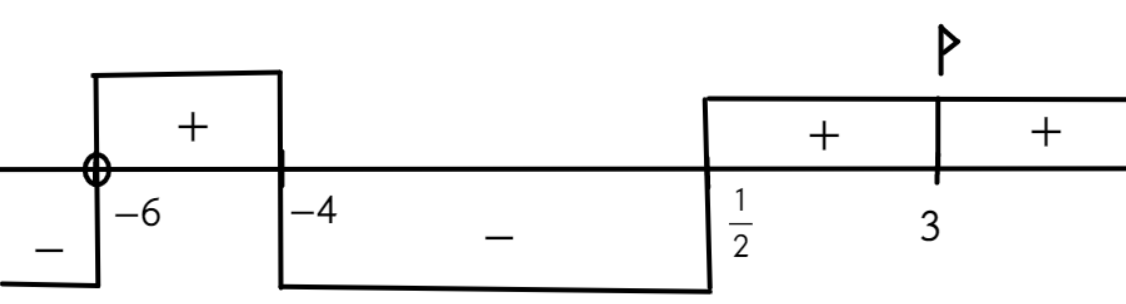
\includegraphics[scale=0.35]{int3.png}}
\end{figure}
$x\in(-\infty; -6)\cup\left[-4;\cfrac{1}{2}
ight]\cup\{3\}.$\\
